\chapter{Determination of the Luminosity Correction} \label{ch:Correction}

\section{Introduction} \label{sec:corrIntro}
The goal of the luminosity measurement experiment is to find the true measure of proton-proton collisions. The LHC sends billions of protons on a head-head collision in a collection of protons called bunches, among which only some protons collide at a given time to produce secondary particles. PLT, located at about 171 cm away from the interaction point and at rapidity, $\eta$,  of $\sim$ 4, inclusively measures the charged particles. 

Within each filled bunch, the profile of the transverse density of protons is expected to be gaussian. Some protons, however, leak into neighboring bunches as seen in Figure ~\ref{fig:pBXfor}. Furthermore, protons can collide with elements within the beam pipe to produce spurious tracks. Some protons leave the ideal orbit and interact with rest gas atoms as the vacuum is not perfect, which causes secondary particle production resulting in extra tracks. 
Fig. \ref{fig:collcat} shows a schematic of tracks from several sources that can be distinguished via the track parameters--slopes, residuals. Generally, the tracks that PLT detects can be categorized as follows:


\begin{itemize}
    \item [1.] Tracks from IP   {\hfill + lumi}
    \item [2.] Tracks from IP with scatter  {\hfill + lumi}
    \item [3.] Tracks parallel to beam from collision with beam gas and obstructions far away from the IP    {\hfill - extra}
\end{itemize}







% draw collision categories
\begin{figure}[htbp!]
\centering
%\resizebox{<horizontal size>}{<vertical size>} {
%\resizebox{scale=0.8}{scale=0.8} {
    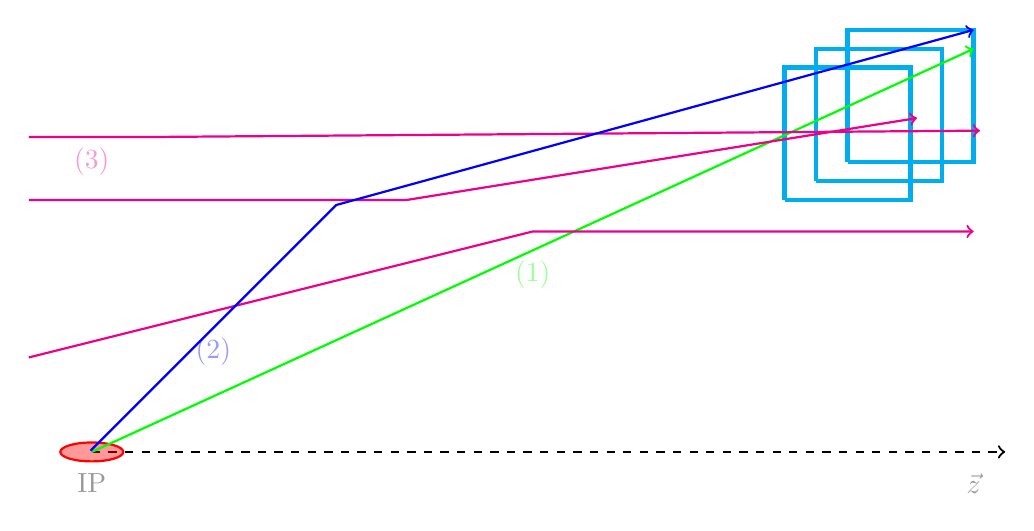
\begin{tikzpicture}[thick,fill opacity=.4,draw opacity=1,scale=0.8]
     %three planes
      \draw[ultra thick, cyan] (11,4) -- (13,4) -- (13,6.1) -- (11,6.1) -- (11,4);
      \draw[ultra thick, cyan] (11.5,4.3) -- (13.5,4.3) -- (13.5,6.4) -- (11.5,6.4) -- (11.5,4.3);
      \draw[ultra thick, cyan] (12,4.6) -- (14,4.6) -- (14,6.7) -- (12,6.7) -- (12,4.6);

      % axes, IP
      \draw [->, black, dashed] (0,0) --(14.5,0);
      \node at (14,-0.5) {$\vec{z}$};
      \draw[fill=red, red] (0,0) ellipse (0.5cm and 0.15cm);
      \node at (0,-0.5) {IP};


      % tracks
      % ++ is addition to last coordinates
      \draw [->, green] (0,0) -- node[below] {(1)} ++ (14,6.4);

      \draw [->, magenta] (-1,5) -- node[below] {(3)} ++ (2,0) --  (14.1,5.1);
      \draw [->, magenta] (-1,4) -- (5,4) -- (13.1,5.3);

      \draw [->, magenta] (-1,1.5) -- (7, 3.5) -- (14,3.5);

      \draw [->, blue] (-0.02,0.02) -- node[below] {(2)} ++ (3.9, 3.9) -- (14,6.7);

    \end{tikzpicture}
            \captionsetup{format=hang}
    \caption{Different sources for tracks entering the PLT during proton-proton collisions. IP refers to interaction point and is the origin of genuine tracks responsible for luminosity.}
    \label{fig:collcat}
%}
\end{figure}

Two different procedures were applied for quantifying the correction term due to accidental tracks for luminosity in 2015 and 2016. Early 2015 data was compromised by the "bug" introduced during the firmware update. Algorithms used to replicate the effect in the luminosity measurement introduced by the bug will be described in section \ref{sec:firmware}, firmware issue. Procedures used to find the corrections based on track parameters for 2015 and 2016 are described in section  \ref{sec:5sigcut} and section \ref{sec:mlfit} respectively.



For the 2016 data, vdm scan data was used as a baseline to define track parameters. During vdm scan, 32 bunches are made to collide out of 3564 bunches. This means there is a very small chance of the measured events to have originated from the secondary collision as mentioned earlier. Section \ref{sec:mlfit} describes the theory behind the maximum likelihood fit method used to parametrize track parameters from the vdm scan and section \ref{sec:highlumifit} provides the resulting fit to higher luminosity regime to assign a correction as a function of luminosity itself.

%move it ahead of fitting procedure?
\section{Firmware Issue} \label{sec:firmware}

%\subsubsection{Double Columns}

On July 31, 2015, a software bug got introduced while making a firmware update which affected how Fast-OR recognized more than 3 hits on a plane. A hit on a given plane corresponds to a charge deposit above a threshold. This charge is translated into a numerical value by the ADC in the FED. The charge deposits in every other double column are added together. Up to three levels of this signal can be distinguished to arrive at a multiplicity count inside the detector plane. The ADC value range is smaller than the dynamic range of the possible charge deposits of more than 2 hits and hence saturates. Instead of repeating the highest saturation value at high multiplicity the value was set to zero in the FED with this firmware upgrade. Hence, it reported no hit and even if the other two planes also registered at least one hit the FED would not recognize this as triple coincidence. As a result, the coincidence count underestimated by a small fraction as the likelihood for 3 hits or more on a single plane was low. To correct for this effect it was implemented algorithmically. It was decided with a counting of such cases from the ADC values obtained from a transparent buffer. 



% describe what gain calibration is?

%\newcommand*{\xMin}{0}%
%\newcommand*{\xMax}{26}%
%\newcommand*{\yMin}{0}%
%\newcommand*{\yMax}{6}%
%\begin{figure}
%\centering
%\begin{tikzpicture}
%    \foreach \i in {\xMin,...,\xMax} {
%        \draw [very thin,gray] (\i,\yMin) -- (\i,\yMax)  node [below] at (\i,\yMin) {$\i$};
%    }
%    \foreach \i in {\yMin,...,\yMax} {
%        \draw [very thin,gray] (\xMin,\i) -- (\xMax,\i) node [left] at (\xMin,\i) {$\i$};
%    }
%
%\draw [step=0.5,blue, very thick] (0.25,0.25) grid (5.5,4.5);
%\draw [very thick, brown, step=0.25cm,xshift=-0.25cm, yshift=-0.25cm] (0.25,0.25) grid +(5.5,4.5);
%\end{tikzpicture}
%\end{figure}

To understand the effect of firmware issue, one has to know how FED receives signals of hits from each plane sensor. Every sensor is divided into 52 columns which are grouped into 26 double columns. Column (1,2), (3,4), (5,6) and so forth. Fast-OR records the occurrence of hits on a given double column, checks if there were hits on other two planes, and saves the result as 0/1 based on whether there was a triple-coincidence or not. The firmware undercounted the triple coincidences when one or more panels had more than 3 double columns hits for a given time period. To account for this issue, the correction was described with full pixel data. As this data contains all registered hits the expected Fast-OR rate was calculated with events that had less than 3 hits. This rate can then be compared to accurate counts from the full pixel data to get the correction factor.


%\newpage
%\begin{samepage}

\begin{figure}[htbp!]
\centering
  \includegraphics[width=0.75\textwidth]%
    {figures/FastOr/firmwareRate.png}% picture filename
        \captionsetup{format=hang}
    \caption{Missing Pixel rate from Fill 4444 averaged over 5 minute interval. Missing rate from the transparant buffer is represented by $+$.}
    \label{fig:Miss_Rate}
\end{figure}

%\textcolor{red}{algo1}: count of the total number of double columns.
%
%\textcolor{green}{algo3}: count of double columns with non-adjacent columns
%
%\textcolor{yellow}{algo4}: count of double columns with non adjacent rows,columns
%
%\textcolor{blue}{algo2}: count of non-adjacent double columns


The red points(\textcolor{red}{algo1}) simply counts the number of double columns and is, therefore, higher than the rate from the transparent buffer. This overcounting occurs as adjacent double columns are blinded by choice of the trigger on the readout chip.
The yellow points(\textcolor{yellow}{algo4}) includes the requirement for adjacent columns on both rows and columns and is, therefore, lower than red and lower than the rate from the transparent buffer. This is expected as FED only checks for adjacency requirement on columns.  The green points (\textcolor{green}{algo3}) counts the number of double columns with non-adjacent columns and the blue points (\textcolor{blue}{algo2}) simply counts the number of non-adjacent double columns, both of which undershoot the rate found via the transparent buffer. This simply demonstrates that the trigger based on double columns in the readout chip does not consistently blind adjacent columns. Therefore, an average between algo1 and algo2 had to be found to match the relative rate of missing triple coincidences. This introduces some arbitrariness in the acceptance of the detector. It is included in the calibration constant $\sigma_{vis}$The rate was eventually chosen to be the one taken from the transparent buffer.

%The rate was eventually chosen to be the one taken from the transparent buffer.



%\end{samepage}

%\section{Accidental Correction} \label{sec:Accidental}
%%\newpage
%Define what accidental correction means. Rename it something else?--background?



\section{Accidental Correction}


There are pure noise or random track contributions to the Fast-OR counting in the PLT that need to be subtracted before translating the Fast-OR rate into luminosity as described in sec \ref{sec:lumiMeasurement}. Two different methods were used to identify such and count accidental tracks. 
Section \ref{sec:5sigcut} describes the method used in 2015 where we define accidental tracks as those that fall outside a region in the distribution of track parameters. 
The relative contribution from the sideband populations is used as a relative correction to the luminosity value. 
Section \ref{sec:mlfit} describes an alternative method first applied to 2016 data that uses a maximum likelihood fit to track parameters distribution. 



%pdf at vdm


\subsection{Track Parameters} \label{sec:trackparams}

PLT is positioned so that it accepts tracks that originated at the IP coming at a particular angle. Background tracks are less likely to pass through all three planes of the telescope because of the way plane 0, 1, and 2 are positioned. Still, stray protons could collide with other stray protons to produce secondary particles that pass through all planes of a telescope which can be mistaken for genuine tracks. Sub-particles could also collide with instruments/molecules in the tube to make fake tracks. 

The slope-y of all tracks is expected to be a distribution with a mean close to the telescope's slope against IP and slope-x mean is expected to be close to 0. The goal is to look at the data and see how track parameters change with respect to the parameters from the vdm scan where beams were far separated, and SBIL was close to 0.


\subsubsection{Track parameters at VdM}
Beam conditions for vdM are different than the regular nominal physics operation, with lower beam intensities and a large separation between few dozens of filled bunches. As such, contribution from the background is expected to be lower, esp since the trigger is only set for colliding bunches. Figure \ref{fig:vdm54} shows the number of tracks as a function of beam separation during the "Y1 scan" in 0.5 $\sigma$ steps. Special trigger was employed for vdm scan to collect as many tracks as possible. 32 colliding bunches and 5 con-colliding bunches were triggered for Fill 4954. 
%Tracks from vdm scan at $0mm$ separation were investigated to find the PDF of slope x and slope y. 


\begin{figure}[htbp!]
\centering
  \includegraphics[width=0.8\textwidth]%
    {figures/VdM/VdMFill.png}% picture filename
        \captionsetup{format=hang}
    \caption{Number of tracks vs Beam separation, VdM Fill 4954(2016).}
     \label{fig:vdm54}
\end{figure}

At higher luminosities when the trigger is random and the per instantaneous luminosity is higher, however, non-luminosity contributions as explained in \ref{sec:corrIntro} are expected to increase. The goal is to find this extra contribution to luminosity measurement as a function of luminosity itself. Probability mass function of track parameters slope-x and slope-y was constructed using 50566 tracks reconstructed by applying the triple-hit condition for the $0$ mm separation of beams during VdM separation scan(Y1). Afterward, deviations from the distributions at higher luminosity was investigated to find out the extra tracks that are seen beyond what is seen at vdm. 


\subsection{5 Sigma Cut Procedure} \label{sec:5sigcut}
For the 2015 run period, fill 4444 was chosen as a representative fill where PLT had the least operational issues. Uncertainty to luminosity was assigned by making quality cuts to track parameters. As shown in Figure \ref{fig:44Slope_Y}, a Gaussian was fitted to slopes and residuals, and  tracks falling outside the cut boundaries were investigated. 

%any tracks outside 5 sigmas from the mean is treated as a 'bad' track. Uncertainty from the change in cut is taken into account 

%5 sigma cuts applied to slopes and residuals to get a linear relationship between the accidentals and the SBIL.


\begin{figure}[htbp!]
\centering
  % trim = {<left> <lower> <right> <upper>}
  \includegraphics[width=0.7\textwidth, trim = {0.2cm 0.2cm 0.2cm 0.25cm}, clip]%
    {figures/slink/Fill4444_SlopeY_SigmaCuts.png}% picture filename
        \captionsetup{format=hang}
    \caption{Slope-y from Fill 4444 with sigma cut boundaries.}
    \label{fig:44Slope_Y}
\end{figure}

It was found that applying cuts outside $4.5$ to $5 \sigma$ and $5$ to $5.5 \sigma$ had little impact on the accidental correction. A combined cut of $5 \sigma$ was applied to both slopes and residuals to define a bad track. Table \ref{tbl:accCorr} shows the various cuts applied to slopes and residuals. An uncertainty of 1.5 \% is assigned to accidental definition resulting from the change in cut criteria.

\begin{table}[htp]
\begin{center}
    \captionsetup{format=hang}
\caption{Variation in the measured accidental rate with different sets of cuts in track parameters.}
\begin{tabular}{| c | c | c | c | c |}
\hline
$\vert S_{x} \vert$ cut & $\vert S_{y} - S_{PLT} \vert $ cut & $R_{x}$ cut (cm) & $R_{y}$ cut (cm) & Measured Accidental Rate \\ \hline
0.002 & 0.007 & 0.03 & 0.03 & 11 \% \\ \hline
0.03 & 0.0105 & 0.03 & 0.03 & 8 \% \\ \hline
0.03 & 0.0105 & 0.02 & 0.02 & 10\% \\ \hline
\end{tabular}
\end{center}
\label{tbl:accCorr}
\end{table}%



%\subsection{Consistency of relative luminosity measurements during physics running}


%\section{VdM} \label{ch:vdm}
%\newpage
\subsection{Maximum Likelihood Fits} \label{sec:mlfit}

Suppose that we have a sample of some n number of independent observations $x_{1}, x_{2}, ..., x_{n}$ from a theoretical distribution $f(x | \theta)$ where $\theta$ is the parameter we would like to find. Let $f(x_{1} | \theta)$ be the probability of observing $x_{1}$ data given $theta$ parameter for function $f$. Then, the probability of observing $x_{1}, x_{2},...,x_{n}$ data is given by the \emph{likelihood} function

\begin{equation}
L(\theta | x) = f(x_{1} | \theta) f(x_{2} | \theta) \cdot \cdot \cdot f(x_{n} | \theta)
\end{equation}

Since we have $x_{1}, x_{2},...,x_{n}$ data and we would like to know what $\theta$ is, L is maximized by 
$$
\frac{dL}{d\theta} = 0
$$

For distributions of the exponential nature, maximum of  the logarithm of L can be found via
$$
\frac{d(lnL)}{d\theta} = 0
$$
The solution to $\hat{\theta}$ is the maximum likelihood $estimator$ for parameter $\theta$ for a given sample. For other samples, $\hat{\theta}$ could be different and thus  $\hat{\theta}$ is a probability distribution. The standard deviation on  $\hat{\theta}$ gives the size of the error in our estimation for true  $\theta$.



%Bin widths are chosen to be smaller than the experimental resolution.

\subsubsection{Likelihood Fit of slope-x at vdm}

The alignment of telescopes is such that there is no preference for slopes to have a particular slope in the x-direction if a track truly originates from the interaction point.

$$
VdM \textunderscore X = {\color {cyan}Gaussian_{core}(\sigma_{1}, \mu_{1})} + f_{1}* {\color {green} Gaussian_{outlier}(\mu_{2},\sigma_{2})}
+ f_{2} * {\color {red} Gaussian(\mu_{3},\sigma_{3})}
$$


\begin{figure}[htbp!]
\centering
  \includegraphics[width=0.7\textwidth]%
    {figures/VdM/VdMSlopeXModel.png}% picture filename
        \captionsetup{format=hang}
            \captionsetup{format=hang}
    \caption{SlopeX model using reconstructed tracks from vdm scan at nominal separation.}
    \label{fig:VdM_Xmodel}
\end{figure}

Fig \ref{fig:VdM_Xmodel} shows the model used for the $x$-slope of the tracks during VdM Y1 scan Fill 4954. The main signal is dominated by a core Gaussian (red), a broader gaussian (green) and yet another gaussian (dashed blue) that spans the range of $x$-slope. The mean value for all the pdfs is close to zero, which is due to the fact that there is no reason for a track to have any preference in the $x-y$ plane.

% group slope-x and slope-y together?

\subsubsection{Likelihood Fit of slope-y at vdm}

The middle plane of each telescope is placed 0.102 cm higher(lower) than first(third) plane. Since the length of telescope is 7.5 cm, the $y$-slope of the telescope itself is around 0.027 which is what $y$-slopes of tracks is expected to be on average.

\begin{figure}[htbp!]
\centering
  \includegraphics[width=0.6\textwidth]%
    {figures/VdM/VdMSlopeYModel.png}% picture filename
        \captionsetup{format=hang}
    \caption{SlopeY model using reconstructed tracks from vdm scan at nominal separation.}
    \label{fig:VdM_Ymodel}
\end{figure}


Fig \ref{fig:VdM_Ymodel} shows the 3 gaussian fit to the slope-$y$ data from VdM Fill Y1 scan. The main signal is dominated by the core gaussian centered at around $0.027$, another gaussian, and one bifurcated gaussian with large $\sigma_{1}$ and $\sigma _{2}$. 

$$
VdM \textunderscore Y = {\color {cyan}Gaussian_{core}(\sigma_{1}, \mu_{1})} + f_{1}* {\color {green} Gaussian_{outlier}(\mu_{2},\sigma_{2})}
+ f_{2} * {\color {red} BiGaussian(\mu_{3},\sigma_{31},\sigma_{32})}
$$





\subsubsection{Combined Fit}
A combined model is constructed using the parameters fixed for both slope-$x$ and slope-$y$ with an extra pdf on top of vdm-$x$ and vdm-$y$ models. The extra contribution to the pdf is allowed to float with a common fraction f for both slopes. Figure \ref{fig:combinedModel} shows the combined fit to one sample data from a regular fill. Both slope-$x$ and slope-$y$ have a predefined shape of the signal taken from the individual fits to slope-$x$ and slope-$y$.

%Both slope-x and slope-y parameters are fed into a model and asked to fit to the VdM data. Ideally, this should produce the null result which is what we find. We then use the parameters and add extra pdf on top of slope-x and slope-y models separately.



$$
Combined \textunderscore Fit = \left ( {\color {green}VdM\char`_X} + f* {\color {magenta} Extra \textunderscore x} \right ) \times \left( {\color {green}VdM\char`_Y} + f* {\color {magenta} Extra \textunderscore y} \right)
$$

\subsection{Fit Validation}
For each individual fit to slopes, different distributions were tested, including gaussian, polynomials, and double Gaussians. For slope-$x$, for instance, a double gaussian eventually converged back to a gaussian. 

As mentioned earlier, there were 50566 reconstructed tracks from the vdm scan. Some of these tracks, however, came from the non-colliding bunches (5 out of 37 triggered bunches were colliding bunches). The Same fit was done for tracks from colliding and non-colliding bunches separately and it was found that there was not much difference in the fit parameters with the changes. 

%Probability mass function
%For each fit to slopes, each PDF was chosen after careful 
%
%The combined model was then fitted to the reconstructed tracks from vdm which assigned 0 fraction to the "extra" stuff which gave a confirmation of the combined model. Furthermore, fitting the model to tracks from only the colliding bunches also gave fraction 0.
%
%separated colliding and non-colliding bunches and made a fit. Didn't change much.
%tweaked gaussians ==> converged to earlier.
%monte carlo simulation







\section{Results} \label{sec:highlumifit}

\begin{figure}[htbp!]
  \includegraphics[width=1.0\textwidth]%
    {figures/VdM/CombinedFit_II.png}% picture filename
    \caption{Combined Fit to the Model.}
    \label{fig:combinedModel}
\end{figure}

The combined model is then fitted to reconstructed tracks from regular fills at higher luminosities.  A bifurcated gaussian is used as an extra pdf for slope-$y$, and a regular gaussian was used as an extra pdf on top of the slope-$x$ model. Figure \ref{fig:correction} shows the increase in the area under the magenta curve as a function of SBIL. The blue line, 2.2\% + SBIL * 1.4\%, is from correction to 2015 data where $5 \sigma$ cut was applied to slopes and residuals. The black dots which increase with a slope of $0.82$ as a function of SBIL, is from 2016 data where likelihood fit method was applied. The fitted line to the black dots goes all the way back to 0, which is the vdm scan with very low value for SBIL. The dotted lines around the black dots represent the uncertainty in the frac3. 

%Since slope from likelihood fit grows slower




%\section{Results}


\begin{figure}
\centering
  % trim = {<left> <lower> <right> <upper>}
  \includegraphics[width=0.8\textwidth, trim = {2.5cm 7.2cm 2.5cm 5cm}, clip]%
    {figures/VdM/correction.pdf}% picture filename
    \captionsetup{format=hang}
    \caption{Coorection as a function of Single Bunch Instantaneous Luminosity (SBIL). The dashed line correspond to the error bars in fraction of non-lumi contribution.}
    \label{fig:correction}
\end{figure}


%colliding bunches only to understand the sensitivity of combined model 
%if the combined fit assigns some fraction f. This made almost no difference i.e. the combined model agrees with the 



%\subsubsection{Residuals}
%
%% describe what residuals mean
%
%\begin{figure}[htbp!]
%\centering
%  % trim = {<left> <lower> <right> <upper>}
%  \includegraphics[width=0.8\textwidth, trim = {0cm 12cm 23cm 0cm}, clip]%
%%  \includegraphics[width=0.7\textwidth]%
%    {figures/VdM/resSample.png}% picture filename
%    \caption{Sample residual distribution for slope-y from combined fit}
%    \label{fig:Res_Ymodel}
%\end{figure}
%
%
%\subsection{Systematics}
%For each slopes, several pdfs were used with floating fraction. The pdf for slope-x and slope-y that we used finally was found to be the most significant.
%
%\begin{itemize}
%\item Validate fit with Toys
%\item cross check: fit VdM ddata with full model $\rightarrow$  fits $f = 0$
%\item systematic uncertainty - shape variation
%\item try two gaussians with well separated mean (and sigma) instead of single gaussian --when floated coverges back to single gaussian(bigaussian)
%\item single gaussian and bigaussian interchanged
%\item fix widths to values of measurements at comparable luminosity
%\item Let VdM core Gaussian parameters float
%\end{itemize}


\subsection{Toy Monte Carlo Simulation}

A monte-carlo toy simulation was performed to understand the relationship between the accidental cut applied for 2016 data and the fraction of the magenta curve from the likelihood fit. For a sample Fill, 100,000 tracks were generated with parameters from the combined model and the fraction of magenta was fixed to some value. A single gaussian was fitted to slope-$x$ and slope-$y$ separately, and the sigma and mean was extracted. Afterward, the number of tracks falling outside the 5$\sigma$ cut on slope-$x$ and slope-$y$ was calculated multiple times for a given fraction3. The result is shown in figure \ref{fig:montecarlo} and it shows a linear relationship between the area under the magenta curve and the 5 sigma cut. The slope from the fit is 0.82, and the intercept is 7.63. Slope less than 1 implies that the area under magenta curve increases faster than the area outside the 5 sigma cut.
%The slope of $0.82$ implies that the area under magenta curve grows faster than the area under the 5 sigma cut.


\begin{figure}[htbp!]
\centering
  % trim = {<left> <lower> <right> <upper>}
  \includegraphics[width=1.0\textwidth, trim = {1cm 2.5cm 1cm 1.5cm}, clip]%
%  \includegraphics[width=1.0\textwidth]%
    {figures/VdM/mc.png}% picture filename
        \captionsetup{format=hang}
%    \caption{Fit model reconstruction of tracks outside $5 \sigma$}
\caption{Extrapolation of fit model to high accidental fractions vs the counting of the track in tails (outside $5 \sigma$) variable distributions.}
    \label{fig:montecarlo}
\end{figure}

It should be noted that the 5 sigma cut applied for 2015 data was on both the slopes and residuals.  Maximum likelihood fit was done for the relevant independent variables, the slopes, and residuals are simply taken as a measure of track quality. A correction was then applied to the 5 sigma cut procedure that was applied to 2015 data. 




%\begin{table}
%\begin{center}
%    \begin{tabular}{| l | l | l | l |}
%    \hline
%    {\bf Interaction} & {\bf Strength} & {\bf Theory} & {\bf Mediator} \\ \hline
%    Strong & 10 & Quantum Chromodynamics & Gluon \\ \hline
%    Electromagnetic & $10^{-2}$ & Quantum Electrodynamics & Photon \\ \hline
%    Weak & $10^{-3}$ & Flavordynamics &  W and Z Bosons\\ \hline
%    Gravitation & $10^{-42}$ & Geometrodynamics & Graviton \\
%    \hline
%    \end{tabular}
%     \caption{Rough order of the interaction strengths, the mediator and the theory, which describes
%these interactions}
%
%\end{center}
%\end{table}


\section{Conclusion}


I built data pipelines for real-time data visualization and monitoring, wrote alarm system for anomalies detection by inspecting time-series data. I also wrote codes to make event reconstruction, analysis code to make statistical models for classification and prediction of  signal and background events in data sets.

Correction to the luminosity measurement by the Pixel Luminosity Telescope (PLT) for the CMS experiment at the Large Hadron Collider was calculated for 2015 and 2016 run period using data-driven statistical methods. The result from likelihood fits was used to improve the background subtraction from nonluminosity contributions.
